---
id: tkz-euclide-ejemplo-62
title: "Circunferencia por tres puntos y sector circular"
description: "Creación de una circunferencia por tres puntos y sectores circulares"
keywords: [circunferencia, sector, circular,taller4]
tags: [tkzDrawCircle,tkzDefTriangle,tkzFillSector,tkzFillPolygon]
sort: 62
---
\documentclass[tikz,border=2mm]{standalone}
\usepackage{xcolor}
\usepackage{tkz-base}
\usepackage{tkz-euclide}

\begin{document}
    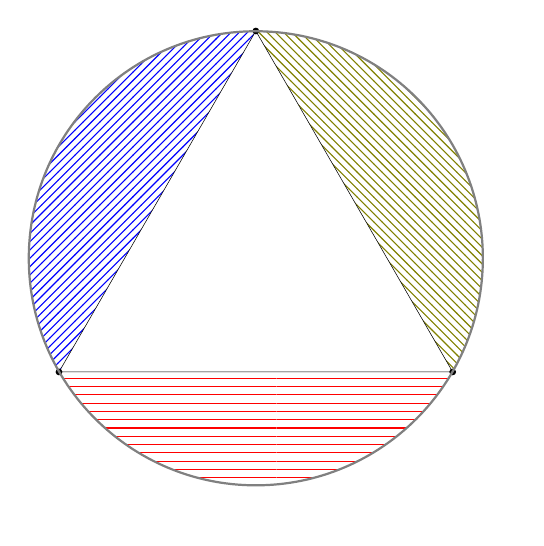
\begin{tikzpicture}
        % Paso 1: Define puntos de la base del triángulo PQR.
        \tkzDefPoint(9,3.5){P}
        \tkzDefPoint(14,3.5){Q}

        % Paso 2: Define triángulo equilátero y encuentra punto R
        \tkzDefTriangle[equilateral](P,Q) \tkzGetPoint{R}        
        
        % Paso 3: Define círculo cuya circunferencia pasa por PPR
        % y determina el centro S del círculo.
        \tkzDefCircle[circum](P,Q,R) \tkzGetPoint{S}

        % Paso 4: Rellena el sector circula SR->P con líneas azules
        \tkzFillSector[pattern=north east lines, pattern color=blue](S,R)(P)

        % Paso 5: Rellena el sector circula SQ->R con líneas color oliva
        \tkzFillSector[pattern=north west lines,pattern color=olive](S,Q)(R)

        % Paso 6: Rellena el sector circula SP->Q con líneas color rojo
        \tkzFillSector[pattern=horizontal lines, pattern color=red](S,P)(Q)

        % Paso 7: Rellena de blanco el polígono del triángulo PQR
        \tkzFillPolygon[white](P,Q,R)

        % Paso 8: Dibuja los puntos del triángulo PQR
        \tkzDrawPoints(P,Q,R)
        
        % Paso 9: Dibuja el polígulo triangular PQR
        \tkzDrawPolygon(P,Q,R)
        
        % Paso 10: Dibuja la circunferencia SP
        \tkzDrawCircle[thick](S,P)        
    \end{tikzpicture}
\end{document}